\section{Discussion}

\begin{frame}
    \frametitle{Points forts de RoBERTa}
    \begin{itemize}
        \item Compréhension fine des sentiments : RoBERTa excelle dans la compréhension fine des sentiments exprimés dans les avis, en distinguant clairement entre les sentiments positifs, négatifs et neutres.

        \item Capacité à identifier les tendances : RoBERTa peut découvrir les tendances émergentes dans les avis, y compris les préférences alimentaires, les aspects appréciés ou critiqués, offrant ainsi des informations précieuses sur les évolutions du marché.

        \item Analyse de mots clés et d'expressions fréquemment utilisés : RoBERTa peut aider à déterminer les aspects importants en analysant les mots clés et les expressions fréquemment utilisés dans les avis, permettant une identification rapide des points forts ou des points faibles des produits.
    \end{itemize}
\end{frame}


\begin{frame}
    \frametitle{Limites de RoBERTa}
    \begin{itemize}
        \item Dépendance aux données d'entraînement : RoBERTa dépend fortement des données sur lesquelles il a été formé, ce qui peut affecter sa précision.
        \item Interprétation des résultats : Les modèles NLP complexes comme RoBERTa peuvent être difficiles à interpréter, rendant délicate l'interprétation des résultats.
        \item Besoin de ressources informatiques importantes : RoBERTa nécessite des ressources informatiques importantes pour son utilisation.
    \end{itemize}
\end{frame}
\begin{frame}
    \frametitle{Limites de RoBERTa}
    \begin{itemize}
    
        \item Des Textes mal Classés : Malgré la plupart des classifications correctes, il peut y avoir des textes mal classés en raison de nuances linguistiques.
        
        \begin{figure}[h]
            \centering
            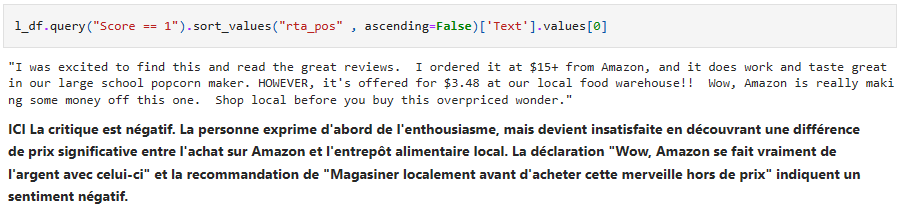
\includegraphics[scale=0.4]{Figures/pointsfaible1.png}
            \caption{Limites de RoBERTa : Example 1 }
            \label{fig:Limit1RoBERTa}
        \end{figure}

        \begin{figure}[h]
            \centering
            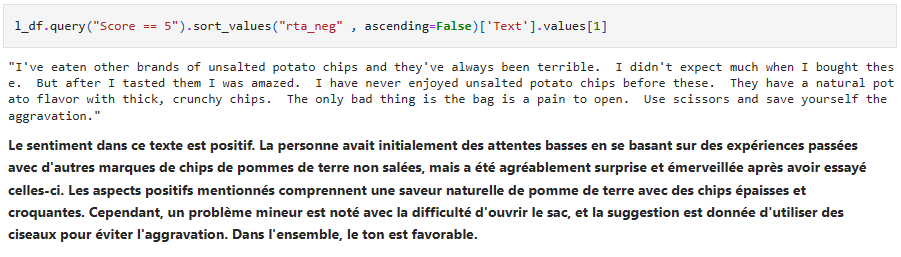
\includegraphics[scale=0.3]{Figures/pointsfaible2.png}
            \caption{Limites de RoBERTa : Example 2 }
            \label{fig:Limit2RoBERTa}
        \end{figure}
        
    \end{itemize}
\end{frame}

\begin{frame}
    \frametitle{Suggestions et améliorations possibles du projet}
    \begin{itemize}
        \item Exploration de sous-catégories alimentaires : Explorer les sentiments dans des sous-catégories spécifiques de produits alimentaires pour obtenir des informations plus détaillées.
        \item Enrichissement du modèle avec des données spécifiques au domaine : Utiliser des données spécifiques au domaine alimentaire pour enrichir le modèle.
        \item Intégration de la rétroaction des entreprises : Permettre aux entreprises de répondre aux avis pourrait offrir une perspective plus complète sur la satisfaction du client.
        \item Analyse de la dynamique temporelle : Investiguer les tendances au fil du temps en analysant les changements mensuels dans les avis.
        \item Comparaison avec d'autres modèles NLP : Comparer avec d'autres modèles NLP pour évaluer la performance relative.
    \end{itemize}
\end{frame}

\begin{frame}
    \frametitle{Implications et conclusions tirées des résultats obtenus}
    \begin{itemize}
        \item Tendance positive globale : La distribution des scores suggère une tendance positive globale dans les avis des clients sur les produits alimentaires d'Amazon.
        \item Importance des avis avec des scores élevés : La majorité des scores sont entre 4 et 5, soulignant l'importance des avis positifs.
        \item Prévalence des évaluations positives : La fréquence élevée des évaluations positives, en particulier avec un score de 5, peut indiquer une propension des utilisateurs à partager leurs expériences positives.
    \end{itemize}
\end{frame}
